\chapter{Related Work}
\label{chp:relatedwork}
This is a research field that has a lot of attention in both academy and industry in past and present years. Hence, the
related work in this area and related fields is quite extensive and broad. With that in mind, we will split this section
in (1) General trajectory data and pattern mining and (2) Flock pattern mining

It is worth noting that the only set of research works that are pertinent to this work, are those at
\secref{sec:rel_flocks}. Hence, those will be the only research works that we will point out flaws that are solved by
this thesis.

\section{General trajectory data and pattern mining}
\label{sec:rel_general}
Here we present the broader scope of Trajectory data mining that were useful to gather some understanding in the field
and insightful ideas for this thesis.

Laube et al. \citep{remo} proposed the REMO concept, which analyzes motion attributes of entities
(speed, azimuth and location) and relate to the motion of other entities that are close to them. They also introduced
some moving patterns, such as flock, convergence, encounter, and leadership. In the end the authors went through some
data structures and algorithms that can be used in order to detect those patterns. However, only high level abstract
algorithms were presented, but neither concrete implementation nor evaluation was shown.

An interesting approach for finding patterns that are frequently repeated by MOs was presented by Cao et al.
\citep{frequentpatterns}. The authors presented an algorithm that focused on approximating the spatio-temporal series
of a MO to a line, where the distance of each trajectory point of that MO to the line would be no greater than a
pre-defined threshold. After that, bounding boxes were created based on those approximated lines and then lines that
belong to the same box are declared as similar sequential patterns.

Algorithms aiming at finding moving clusters, with MOs coming in and out of the cluster, are presented by Kalnis et al.
\citep{movingclusters}. In that research paper, the authors consider a moving cluster as a moving region despite the
identity of the objects that are part of it, but for each time stamp the intersection of points between subsequent
clusters needs to be above a certain threshold $\theta$. In \figref{fig:clusters} one can see a moving cluster composed
by clusters $S_0$, $S_1$ and $S_2$, having $\theta=0.5$, meaning that $\dfrac{|c_i \cap c_{i+1}|}{|c_i \cup c_{i+1}|}
\geq 0.5$. They presented three different approaches to find moving clusters (with one of them being an approximation
method), being supported by a density function. They claim that their proposal are applicable for large-temporal
datasets, but that large dataset that they analyzed had only 50K entries. Yet on clusters, Jensen et al.
\citep{clusters3} added velocity as a parameter in order to help finding moving clusters (using dissimilarity
functions), achieving some improvements in processing time. An approach using a trajectory similarity measure based on
the Hausdorff distance is proposed by Atev et al. \citep{clusters2}, where the sequential order of trajectories is
preserved over time. The authors also present a method aiming at clustering trajectories taking advantage of some
spectral clustering methods. A more recent research \citep{clusters1} proposes a novel type of cluster classification:
Influence-based Moving Clusters (IBMC). The author states that an IBMC consists in a set of moving clusters where each
MO, in each cluster, influences at least another MO in the next immediate cluster. It is shown that space for
discovering IBMC is very extensive and an algorithm for finding the maximal answer is proposed.

\begin{figure}
    \centering
    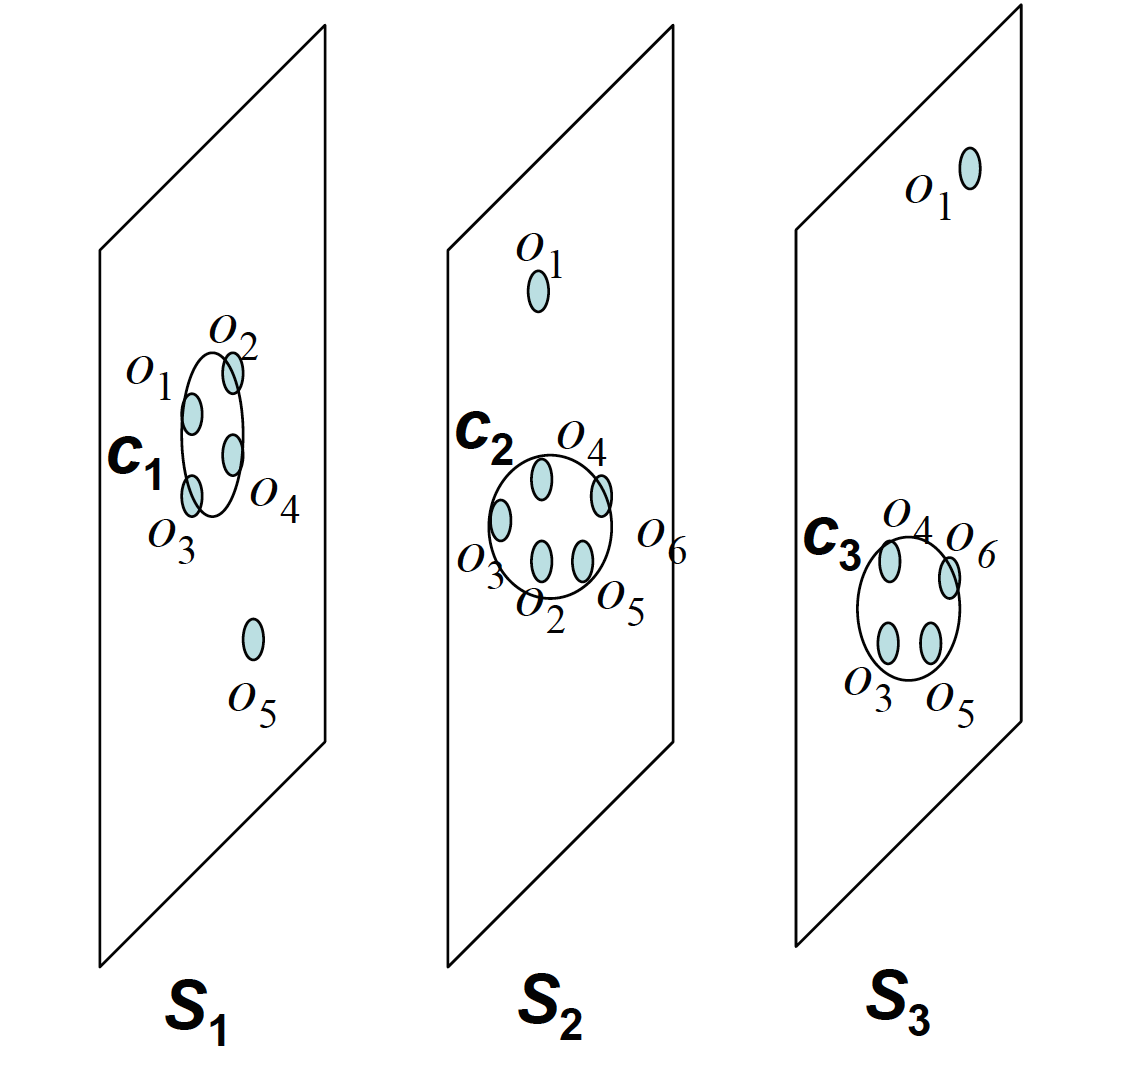
\includegraphics[width=0.5\textwidth]{images/clusters.png}
    \caption{A moving cluster composed by clusters $S_0$, $S_1$ and $S_2$ and $\theta=0.5$ \citep{movingclusters}}
    \label{fig:clusters}
\end{figure}

Jeung et al. proposes the convoy pattern \citep{convoy2}\citep{convoy}. They first point out the key difference between
flock and convoy patterns: Flock pattern relies on all trajectories being present in a disk of pre-defined radius, while
convoy does not rely on any kind of shape to cluster its trajectories. That difference is depicted in
\figref{fig:convoy_pattern}, where the second disk is of different size of the other disks and not all trajectories are
present in the consecutive clusters (another difference from the flock pattern). The authors propose three density based
algorithms to find convoy patterns using line simplification techniques. Their work is inspired by the algorithms
already proposed by \citep{movingclusters} and \textit{DBSCAN} \citep{dbscan}. More work on convoy patterns can be found
by Aung et al. \citep{convoy3}, where they divide convoy patterns in two different groups, namely \textit{Dynamic
Convoys} (DC) and \textit{Evolving Convoys} (EC). To this end, they present three algorithms to identify EC patterns.

\begin{figure}
    \centering
    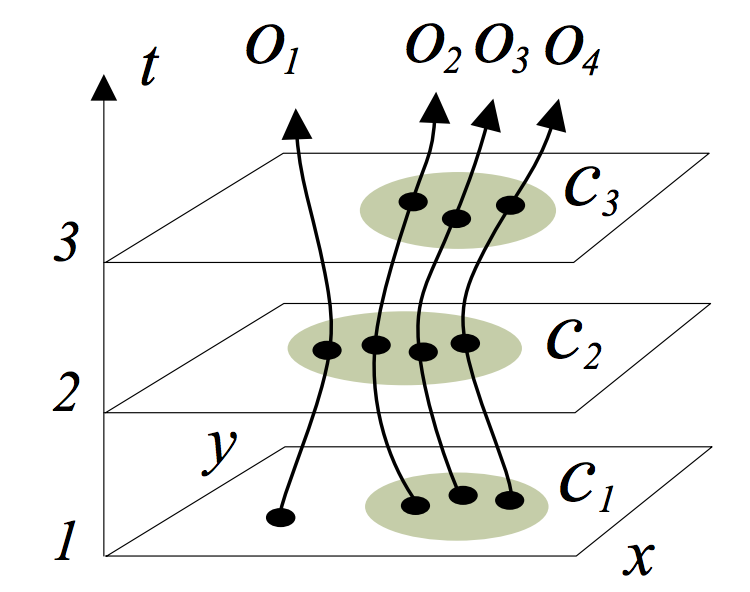
\includegraphics[width=0.5\textwidth]{images/convoy.png}
    \caption{A Convoy pattern \citep{convoy2}}
    \label{fig:convoy_pattern}
\end{figure}

Gathering is another moving pattern that was analysed by the academy. Zheng et al. \citep{gathering} state that a
gathering pattern consists in various group incidents such as celebrations, parades, protests, traffic jams, etc. They
first formalize and model the gathering pattern and then propose algorithms to find the gathering pattern. Effectiveness
and efficiency evaluations are presented showing an overall good result, however only on dataset is analysed. Instead of
looking for patterns that happen exactly at the same time (e.g. clusters and flocks), Li et al. \citep{swarm} propose
the swarm pattern. Such pattern tries to group MOs that may actually diverge temporarily and congregate at certain
timestamps, it is not required also that a trajectory stays all the time with the same swarm cluster. The authors in
that work, formalize the swarm concept and present algorithms to find the pattern. The algorithms effectiveness is
compared against convoy pattern algorithms and it is shown that, for some datasets, the swarm pattern is better suited.

An algorithm to find patterns in Origin-Destination databases, meaning that only the origin and destination points of a
Trajectory are recorded in the analyzed data set, is proposed by Guo et al. \citep{discovering_orig_dest}. They propose
a way to model points of interest, since moving objects going to the same place (e.g. airport) will report different GPS
coordinates. The proposed algorithm has a preprocessing phase that makes a Delaunay Triangulation of the points,
followed by clustering them based two parameters: (k) number of points to build a cluster and ($\theta$) minimum number
of points (or weight) of a cluster. After building the clusters, they derive some mobility measures, in order to extract
spatial and temporal mobility patterns, presenting an useful way of understanding traffic loads in a given city.

Baratchi et al. propose a way to find frequently visited paths between two points of interests. The authors present an
algorithm that deals with trajectory uncertainty and use cluster based techniques to map uncertain trajectories to
actual paths in a map that were most likely to be followed by the moving object. First they gather points of interests
(those where the moving object stayed at least 30 minutes with its speed close to 0) and goup all subtrajectories that
has the same start and end points of interest. They then apply their algorithm, which consists in dividing the space in
grids and assign each point to a grid, and partition those subtrajectories in even small subtrajectories based on
breakpoints. After that partition they use a score mechanism to decide which set of subtrajctories are more likely to be
frequent path. Their algorithm is mainly for offline analysis and uses a map matching algorithm in order to match GPS
points to actual map segments. They did not present the used database nor the numbers of such database. His evaluation
is somewhat shallow and does not present any take away results.

A comprehensive state of the art review in Trajectory Data Mining is presented by Zheng \citep{survey}. He covers
relevant research topics, such as Trajectory data preprocessing, Trajectory data management, Uncertainty of trajectory,
Trajectory pattern mining, and Trajectory classification. He points out some public trajectory datasets that can be used
to evaluate pattern detection algorithms, like the dataset in \citep{tdrive} used in this thesis.

\section{Flock pattern mining}
\label{sec:rel_flocks}
Gudmundsson et al. \citep{gudefficient} \citep{gudlongest} extended and formalized the flock concept proposed by the
REMO Framework \citep{remo}. They also introduced the concept that the flock pattern must contain a disk of radius $R$
in each time step that encloses all trajectories. They proposed approximation and exact algorithms for flock pattern
detection, but no performance evaluations were made and only theoretical analysis were presented, which does not show if
the algorithms are efficient or not. Later on, the same authors \citep{gudlongest} extended the flock pattern definition
by adding the temporal length variable: the entities must stay together during some time interval $\delta$ to be claimed
as a flock. To this end, they presented some approximation algorithms what work on approximating the radius $R$ of the
disk used to cluster the flock, based on a defined $\epsilon$. The evaluations performed \citep{gudlongest} varied only
the $\delta$ parameter leaving all other parameters variation out of the experiments. Additionally, the performance
results were not good, having scenarios where the algorithms took more than 1.5K seconds to analyze a dataset of 1
million entries. It is important to say that all algorithms did waste time by analysing disks that will not form a flock
pattern in the future, thus having a degradation in performance.

Vieira et al. \citep{vieira} proposed a polynomial algorithm to find flock patterns of fixed duration, based in three
parameters: minimum number of trajectories $\mu$, the disk radius $\epsilon$ and a minimum time length $\delta$.  In
order to discover the centers of the cluster disks for each time step, they paired the points that had distance less or
equal to $2*\epsilon$, created two disks based in that pair and tried to cluster other points into those disks. Their
algorithm assumed that each point is sampled in a fixed time interval, assumption that does not reflect real world
datasets. Additionally, their algorithm suffered from wasting CPU cycles by processing disk candidates that are not real
potential flock candidates. The authors also proposed some filtering heuristics to optimize the processing time, but the
optimizations did not present good results, and our local tests showed that the optimizations affected the final number
of flocks found by the algorithm.

An algorithm that mixes together BFE \citep{vieira} with a "Frequent Pattern Mining" heuristic is proposed by Turdukulov
et al.. They make some performance comparison against BFE and were able to show some improvement in the processing time
when varying the radius $R$ of the disk. However, despite the improvements, their results do not propose a fair
comparison: (1) BFE is an on-line algorithm and their implementation imposes an offline implementation; (2) they filter
out some trajectories based on random assumptions (e.g. trajectories with less than 10 minutes or 20 minutes) which
might benefit their algorithm and cut out possible flocks of that length; (3) they only show results varying the disk
radius and not the other parameters used by BFE.

The problem of Maximal Duration Flock Pattern (MFP) is addressed by Geng et al. \citep{enumeration}, proposing
algorithms to enumerate all MFP in a trajectory dataset. MFP, in other words, means that the flock cannot be extended
without increasing the disk radius $R$. They propose a set of algorithms for finding MFP and prove that they can indeed
enumerate all MFP from a trajectory dataset. They also compare their algorithms with BFE from Vieira et al.
\citep{vieira} and show that their implementations outperform the later in some scenarios. However, they still waste CPU
cycles by analyzing disks that will be discarded later, by not being potential flock candidates.

Wachowicz et al. and Wirz et al. \citep{flockpedestrian} \citep{pedestriancanyons} presented algorithms for finding
flocks using pedestrian spatio-temporal data. The former performed a lot pre- and post-processing in the dataset (which
makes not possible to be used in real-time analysis) and neither performance nor accuracy evaluations were presented.
The latter, did not provide any performance evaluation either, only showing accuracy experiments with a tiny dataset of
only 13 entities in a time span of 32 minutes.

Wang et al. \citep{visualtrafficjam} proposes a framework for detecting traffic jams in trajectory data, which can be
considered as a flock pattern, since some moving objects stay together in a road for an interval of time. They list the
requirements for both a data model and a visual interface that their system must have to be able to expose useful
information for users, in order to extract conclusions from the analysis. Their algorithm is bound to a map network,
which means that one part of data preprocessing will be to map the data points to the respective roads in a map. They
claim to be able to detect traffic jams with high accuracy, however they do not have any ground truth data to validate
the assumptions. It is also worth noting that only one dataset is used to evaluate the proposed system, which does not
show that the solution is ready for multiple scenarios.

There are also some work focusing on indoor flock detection using mobile phone sensors, in which Wi-Fi signal strengths
are mapped into coordinates \citep{mobile1}, or a variety of mobile phone sensors (e.g. accelerometer, magnetometer and
Wi-Fi) are used to detect flock patterns \citep{mobile2}. However, those works only address flock detection in indoor
environments, not using GPS coordinates, which are not in the scope of the problem addressed by this thesis.
% * <steniofernandes@gmail.com> 2016-05-26T15:06:57.542Z:
%
% thesis -> phd, dissertation ->master
%
% ^.

\section{Academic Contribution}
It was notorious, from the related work presented in \secref{sec:rel_general} and \secref{sec:rel_flocks}, that there is
a lot to cover in order to provide efficient flock pattern detection as well as an elegant and comprehensive system
architecture to the pattern detection problem (which was not seen in any of the presented works). All of that is a
subject to care about due to the extensive number of scenarios that data pattern mining, as well as flock patterns, can
help and be applied to. We can have flock pattern detection helping, to name a few \citep{applications}:

\begin{enumerate}
    \item \textbf{Traffic Management}: Unusual grouping of vehicles, or abnormal traffic volume in certain regions can
        be detected with help of flock pattern detection algorithms. That information can help the accountable entities
        to better plan cities or traffic spaces.
    \item \textbf{Surveillance and Security}: Suspicious movements of groups of people or vehicles can indicate a
        security threat and automatic pattern detection systems can aid to detect abnormal behavior in a group of moving
        objects.
    \item \textbf{Human Movement}: Governmental organizations can study how people are moving from one part of the
        city/country/state to another with the help of flock pattern detection, for example. They also can gain insights
        about the habits of the population and provide resources to enhance life quality of those involved.
\end{enumerate}

In \secref{sec:architecture} we will propose an elegant and extensible System Architecture that will be able address
almost any pattern detection problem. Such architecture will be divided in logic modules and components, each one with a
very specific and self-contained goal, making then reusable and extensible to address other data analysis problems. We
will also show that by modifying a single component in that architecture will enable the usage of a different software
paradigm, thus proving its modularity, extensibility and ease to use.

We could notice that the presented algorithms suffer from CPU cycles waste by processing data that will not generate any
pattern, like the flock disks that contain points that are not present in subsequent time steps. Avoiding such
unnecessary processing can boost the running time of a flock pattern detection algorithm and then provide information in
a real time fashion for decision takers. With that in mind, we will present an efficient algorithm, based on bitmaps,
that will only be concerned with data that can really generate flock patterns, saving a considerable amount of time and
being able to provide information way faster than other algorithms about the datasets being analyzed. We will prove that
by showing benchmarks comparing the running time of our solution against the state of the art algorithm and also show
how our implementation generates way less unimportant data that dramatically affect the running time of the state of the
art algorithm. Last, but not least, we will provide a multi-core aware implementation of our algorithm, taking advantage
with the system architecture mentioned in the previous paragraph, which will achieve even more savings in running time,
without affecting the number of flocks that are found. Aiming at showing that our solution is ready for multiple types
of data, we will perform experiments with 4 different datasets, being them real and synthetic generated and with a large
amount of data entries, with some of them having more then 50 million entries.
